\section{Result analysis}
\label{sec:results}

    This section will discuss the results drawn from running a great number of tests, consisting of two parts: parties that do not consider the total power of coalitions and agents that do use the power-weighted model.

    \subsection{Parties without power-weighting}

        \subsubsection[Finding a suitable range of the exponent alpha]{Finding the suitable range of the exponent $\alpha$}
            Since the exponential function is used by our party, the next step is to build parties with different exponents and test them in the MOPaC protocol to find the exponent for which the party will have the best performance. \\

            The exponent $\alpha$ as in \autoref{exponential} was varied over the following values: "0.05, 0.4, 1, 3, 9". The relation between the factor with which the utility threshold decreases, 'k', and time are found in \autoref{fig:exp} for all different values of the exponent. \\

            The same figure also shows that an exponent of $\alpha = 1$ leads to a linearly decreasing threshold. The exponents smaller than "1" cause a slow-decreasing result of the exponent function at the beginning which means the party won't accept the bid too easily, and vice versa. Values of the exponent were chosen such that extreme, moderate and neutral patterns were considered, both increasing and decreasing. \\

            To test these parties with different exponents, a program was created to automatically run sessions with all other example parties provided by GeniusWeb: "RandomParty", "Timedependent", "Linear", "Conceder", "Hardliner" and "Boulware". Adding the five exponential parties, 11 parties will be randomly selected to run a session using the "Party" profiles, which means each session contains four teams to negotiate with each other. 4000 repeated sessions were run. The results are plotted in box plots.\\
\begin{comment}
            
            \begin{figure}[H]
                \centering
                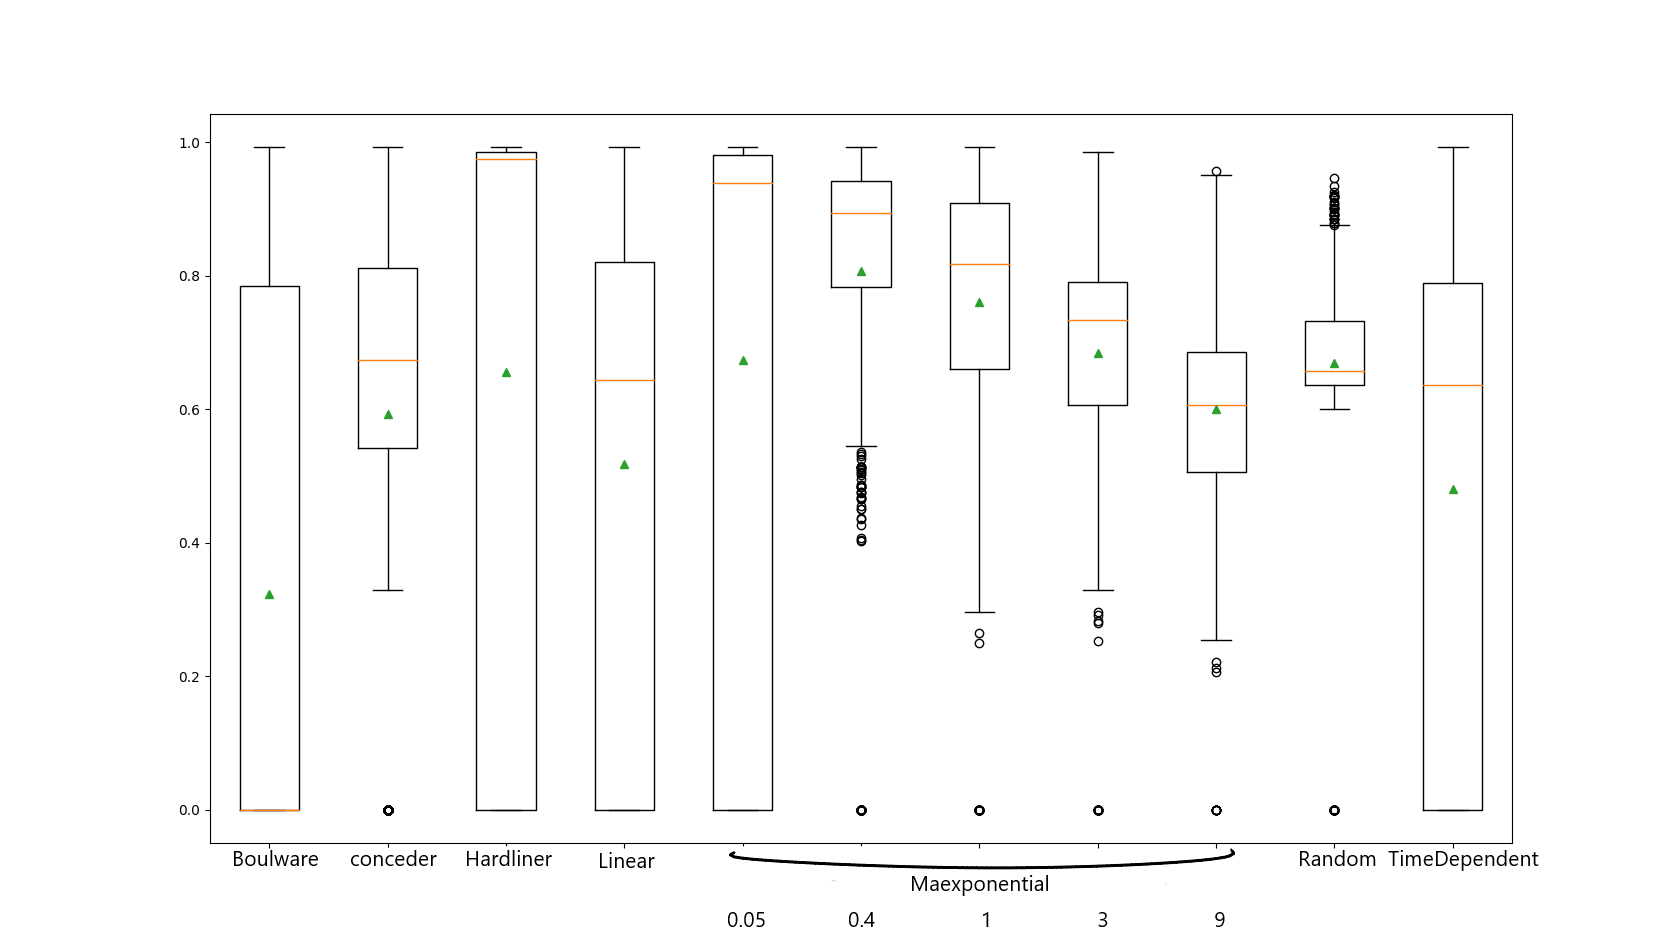
\includegraphics[width=15cm]{figures/Basic_test_1.png}
                \caption{Box plot depicting the utility outcome values for the different parties, after 4000 random sessions. Outcomes without an agreement are included (zero utility).}
                \label{fig:test_1}
            \end{figure}
\end{comment}

            From \autoref{fig:test_1}, it is clear that among the five exponential parties, the mean utility decreases with the increase of the exponent. However, "0.05" with the highest mean utility, performs badly in achieving agreements steadily in these sessions. The long length of the box shows there are large numbers of 0 utility when using "0.05". Then the "0.4" option seems to perform well among these parties. It achieves good balance between the utility and the final agreement. The next step is to seek more possible values around "0.4" to find out the value has the best performance.

        \subsubsection[The optimal value of exponent alpha]{The optimal value of exponent $\alpha$}

            Based on the former result, a second test was executed to find a suitable exponent value in a smaller range. This time the range of $\alpha$ was centered at 0.4 with an interval of 0.1, expanding outward. Considering that "0.05" and "1" were already taken into consideration, the range of the exponent can now be limited. A range of $0.2-0.6$ was selected. The session is repeated only 400 times now. \\

\begin{comment}
            
            \begin{figure}[H]
                \centering
                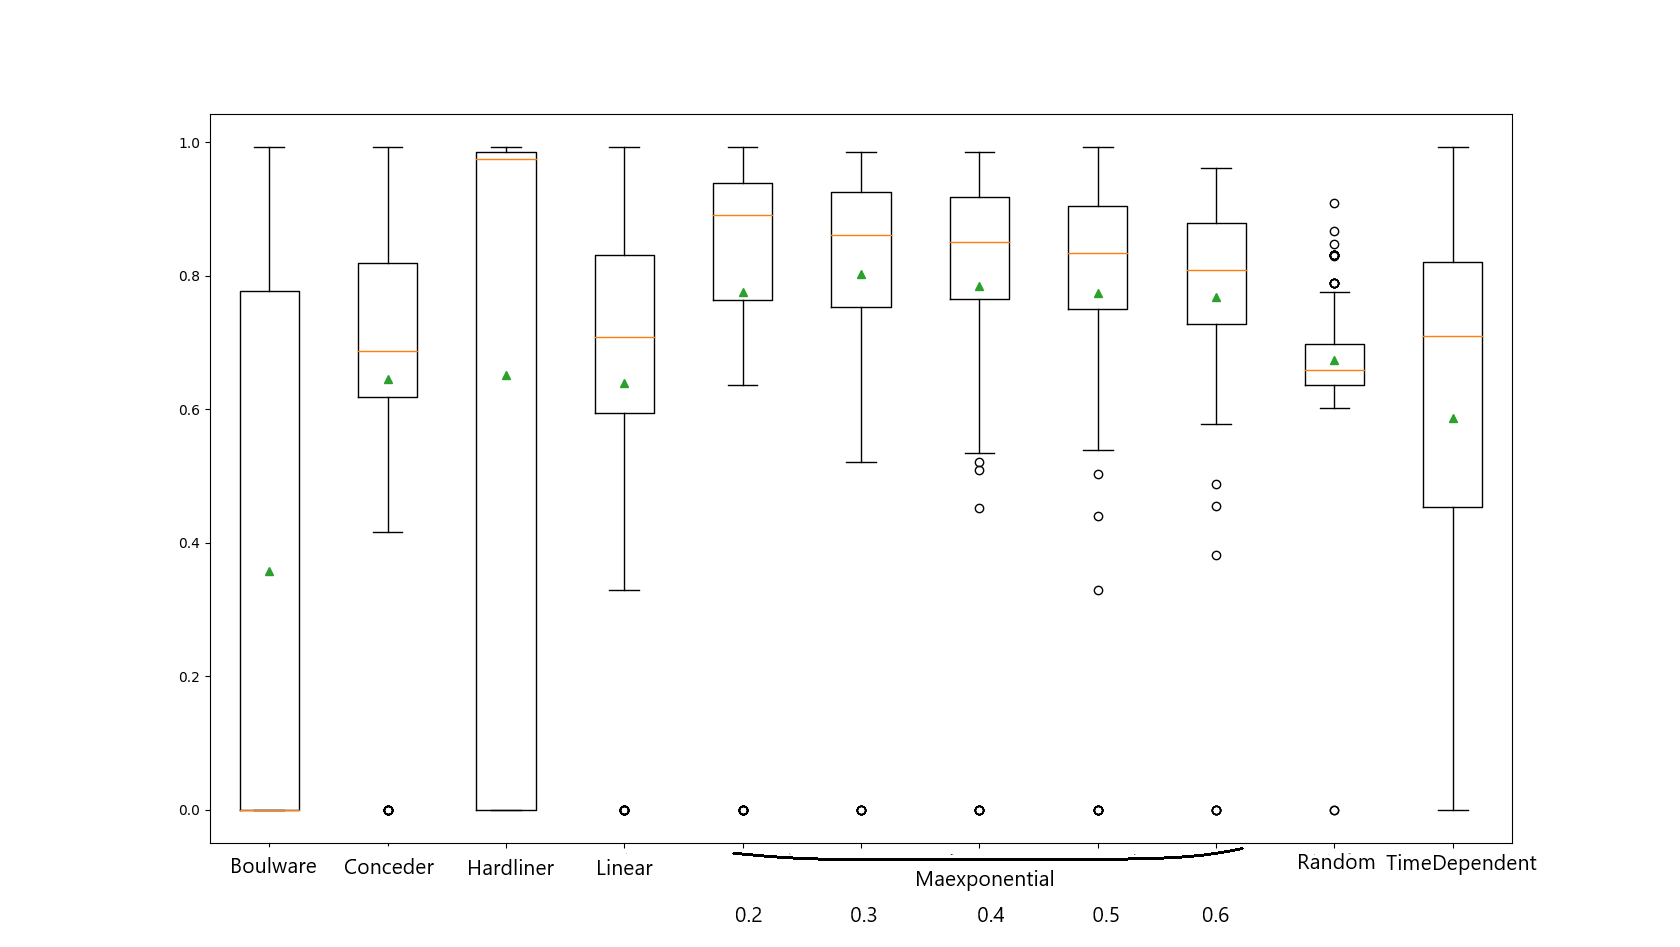
\includegraphics[width=15cm]{figures/Basic_test_2.png}
                \caption{Box plot depicting 400 random sessions with the exponential agents within a smaller range for the exponent (0.2-0.6)}
                \label{fig:test_2}
            \end{figure}
\end{comment}

            According to \autoref{fig:test_2}, the Linear and TimeDependent parties have a more optimal performance now. This probably has to do with the exponential parties in the sessions, that are performing closer to optimal now, leading to more (optimal) agreements for all agents. 
            
            Moreover, the median and box-position of exponential parties are decreasing with increasing exponent value in range: "0.2, 0.3 ,0.4, 0.5, 0.6", which means "0.2" is most suitable value in this test.
            
            In a final iteration, with a step size of only 0.05, results as in \autoref{fig:test_3} were found. the optimal exponent value is found to be $\alpha = 0.15$.   \\

            In summary, compared to other parties, the exponential party can reach relatively many agreements with high utility. Especially in the discussed, optimal ranges of the exponent $\alpha$.

\begin{comment}


        \subsubsection{Value with best performance}

            Finally, a similar test was performed with exponents ranging from $\alpha = 0.1$ to $0.85$, with the step size being 0.05. From \autoref{fig:test_3}, the optimal exponent value is found to be $\alpha = 0.15$. 
           
\end{comment}    
          
            


\begin{comment}
            
            \begin{figure}[H]
                \centering
                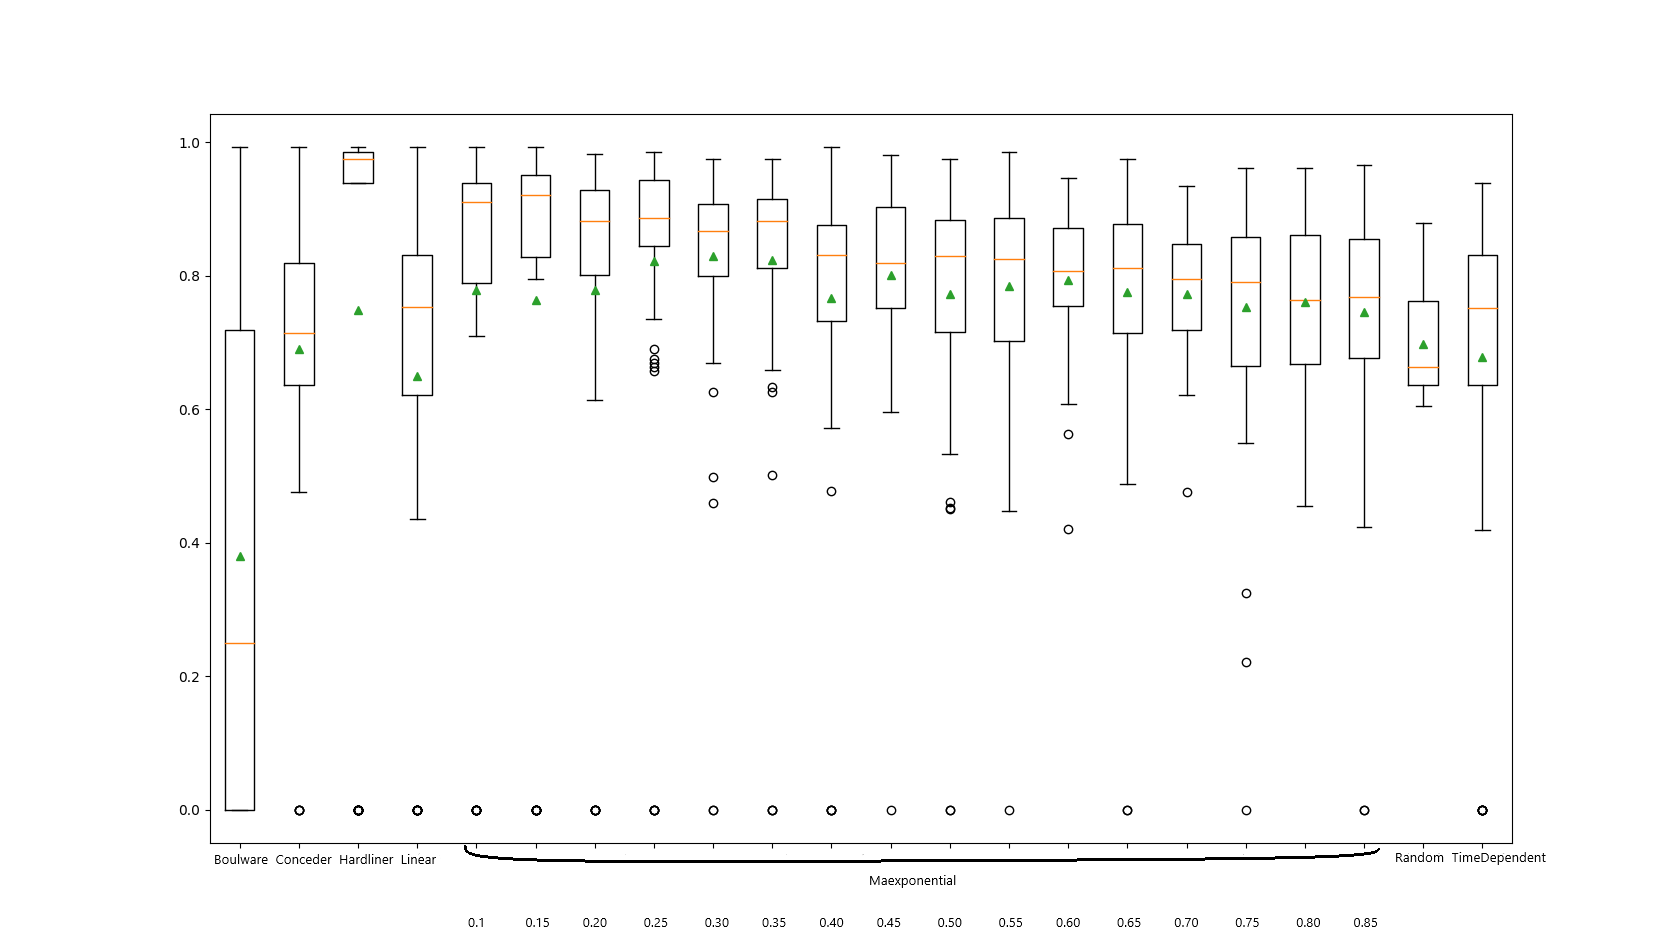
\includegraphics[width=15cm]{figures/Basic_test_3.png}
                \caption{Final box plot depicting the outcome of 400 sessions and $\alpha$ ranging from 0.1 to 0.85 with steps of 0.05.}
                \label{fig:test_3}
            \end{figure}
\end{comment}

    


        \subsection{Parties with power-weighting}
        In \autoref{sec:strategies} the importance and set-up of parties that use power-weighting was discussed. 
        \subsubsection{Power Influence}
        
        \begin{comment}
             
             \begin{figure}[H]
                \centering
                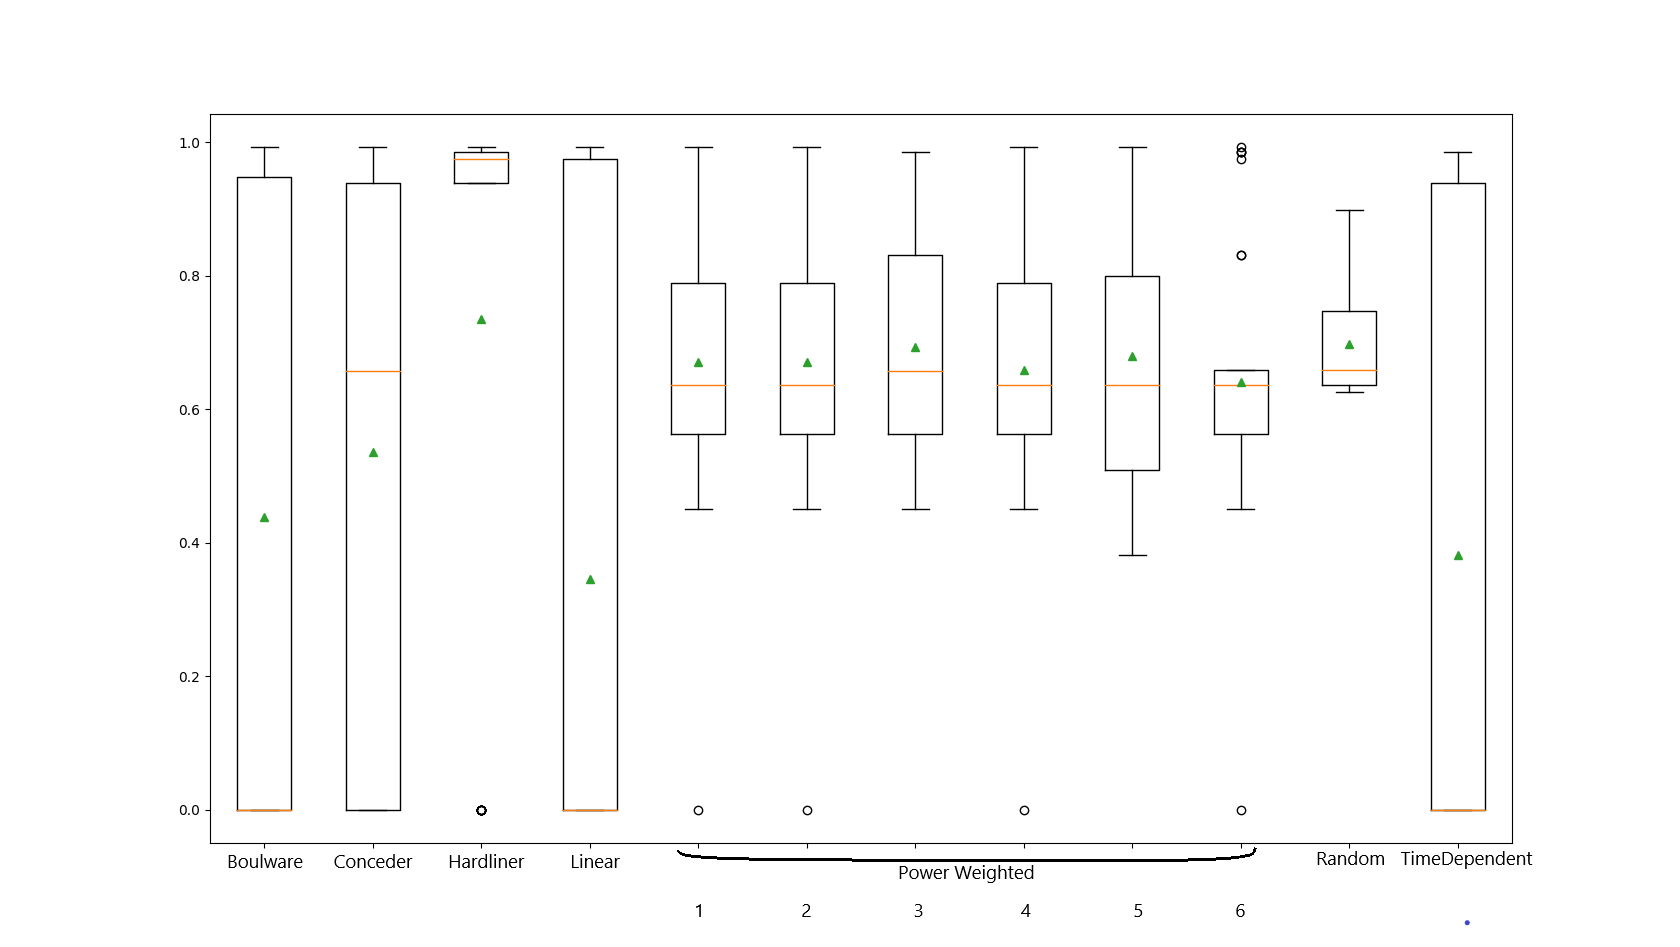
\includegraphics[width=15cm]{figures/Power factor test.png}
                \caption{Power factor test}
                \label{fig:power_factor}
            \end{figure}
        \end{comment}
   
            When referring to variables for the power-weighted models in this and the next section, this is with reference to \autoref{powerpar}.
            In this test, $\alpha$ was set to 0.3 for all "power-weighted" parties, while $\beta$ was set to 1, 2, 3, 4, 5 and 6 for the respective parties. Besides, the other parties' power is set to 1. \autoref{fig:power_factor} shows that setting different values of $\beta$, thus changing the importance of power-weighting, does not seem to influence the performance of the agent.\\
            
            However, if the GeniusWeb framework would allow for more agents in the negotations, it is expected to be able to prove a positive influence of the power-weighting on the agent's utility outcome. The ideal value of $\beta$ in this case is hard to predict.
            
            
            
       \subsubsection{Power Influence with time}
       
       
       \begin{comment}
       
       \begin{figure}[]
                \centering
                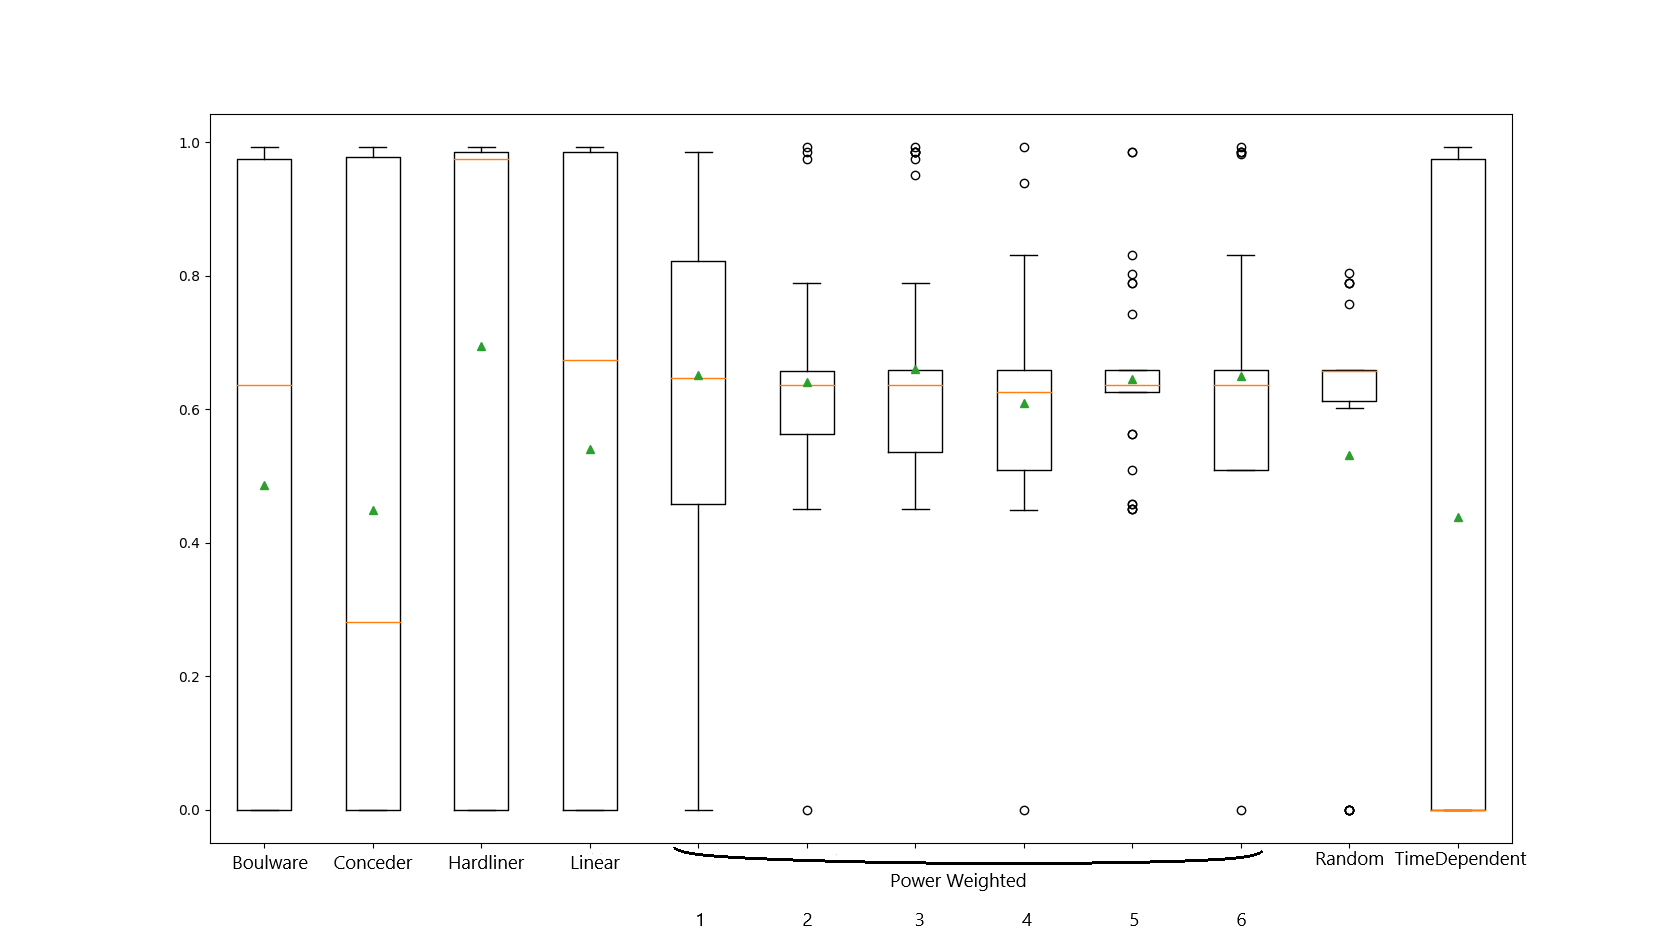
\includegraphics[width=15cm]{figures/Power-Time.png}
                \caption{Power factor test}
                \label{fig:power_time}
            \end{figure}
              \end{comment}

       For this final test, the value of $\alpha$ was varied from $0.2$ to $0.6$ - which varies the influence of the power over time. As in \autoref{fig:power_factor}, the outcome in \autoref{fig:power_time} does not show more than a negligible influence of the different values of $\alpha$. \\
       
       As explained earlier, the power-weighting is expected to have a positive effect on the agent's outcome in negotations with more agents than can be simulated in this GeniusWeb framework. Finally, higher values of $\alpha$ would then be expected to prove more effective, as the influence of power would  increase over time. This simulates the realistic situation in which an agent starts deviating from his favourite products because he sees more chance to join a coalition, only towards the end of a negotiation. 
        
